
\section{Introduction}
\label{sec:introduction}
%%% General intro
\PARstart{T}{he} exponential improvement in computing performance and the availability of large amounts of data are boosting the use of artificial intelligence (AI) applications in our daily lives. Among the various algorithms developed over the years, neural networks (NNs) have demonstrated remarkable performance in a variety of image, video, audio, and text analytics tasks \cite{schmidhuber2015deep,Taigman_2014_CVPR}. Historically, artificial neural networks (ANNs) can be classified into three different generations \cite{Design_Exploration_SbS_Trans20}: the first one is represented by the classical McCulloch and Pitts neuron model using discrete binary values as outputs; the second one is represented by more complex architectures as multi-layer perceptrons (MLPs) and convolutional neural networks (CNNs) using continuous activation functions; while the third generation is represented by spiking neural networks using spikes as means for information exchange between groups of neurons. Although the AI research is currently dominated by deep neural networks (DNNs) from the second generation, \deleted{nowadays} the SNNs belonging to the third generation are receiving considerable attention \cite{Spinnaker_Trans13,ernst2007efficient,Design_Exploration_SbS_Trans20, SNN_Survey_Trans19}.

SNNs offer advantageous robustness and the potential to achieve a power efficiency closer to that of the human brain.
%%%
\REVIEW{SNNs operate reliably using stochastic elements that are inherently non-reliable mechanisms \mbox{\cite{mcdonnell2011benefits}}.
This provides superior resistance against adversary attacks
	\mbox{\cite{ernst2007efficient, Dapello2020.06.16.154542}}. Beside
robustness, SNNs have further advantages like the possibility of a more efficient asynchronous parallelization and higher
energy efficiency than DNNs. For
example, Loihi \mbox{\cite{davies2018loihi}}, a SNN developed by Intel, can
solve LASSO optimization problems with an over three orders of
magnitude better energy-delay product than conventional
approaches. These advantages are motivating large research programs by
major companies (e.g. Intel \mbox{\cite{davies2018loihi}} and IBM
\mbox{\cite{TrueNorth_Trans15}}) as well as pan-european projects in the
domain of spiking networks \mbox{\cite{Spinnaker_Trans13}}, and
attempts to transfer features from SNNs to standard DNNs
\mbox{\cite{pfeiffer2018deep}}.
}

\REVIEW{SNNs emulate the real behavior of neurons in different levels of detail. The more detailed the biological part is emulated, the greater the computational complexity \mbox{\cite{izhikevich2004model,amunts2019human}}. Most of today's SNNs use a very detailed model. In contrast, Spike-By-Spike (SbS) neural networks are on the less realistic side of the biological realism scale \mbox{\cite{rotermund2019Backpropagation,ernst2007efficient}}. In spite of that, SbS still uses stochastic spikes as a means of transmitting information between populations of neurons, and thus retains the robustness advantages of SNNs. Correspondingly, the hardware complexity of the approach is greatly reduced
  \mbox{\cite{nevarez2020accelerator,rotermund2018massively}}.
}


%%% SbS intro
%SbS neural networks \cite{rotermund2019back,ernst2007efficient} are inspired by the %natural information processing of the mammalian brain.
The conceptual model in SbS (see \mbox{\sect{sec:sbs}} for a short review) differs fundamentally from conventional ANNs since (a) the building blocks of the network are inference populations (IP) which are an optimized generative representation with non-negative values, (b) time progresses from one spike to the next, preserving the property of stochastically firing neurons, and (c) a network has only a small number of parameters, which is an advantageous noise-robust stochastic version of Non-Negative Matrix Factorization (NNMF). \REVIEW{As discussed in \mbox{\sect{sec:sbs}}, SbS incorporates the inherent robustness of SNNs and the regular flow of information from CNNs.} These properties place the SbS network in between non-spiking NN and stochastically spiking NN, offering advantages from both worlds \cite{rotermund2019Backpropagation}.  


%%%%%%% Problem statement
\REVIEW{The computational demands of ANNs, and in particular SNNs, must be addressed by specialized hardware architectures. A significant research effort has been performed in SNN accelerators, see e.g.
  \mbox{\Refs{roy2019towards,bouvier2019spiking,
      young2019review,TrueNorth_Trans15,Spinnaker_Trans13,davies2018loihi}}.
  However, hardware accelerators that focus on SbS have only been partially investigated so far \mbox{\cite{nevarez2020accelerator,rotermund2018massively}}.
  Enhanced SbS accelerators will have a double impact. From an engineering point of view, they will contribute to the deployment of robust neural networks in small embedded systems \mbox{\cite{nevarez2020accelerator}}; from a scientific point of view, they will facilitate experimentation with SbS methods for neuroscience
  \mbox{\cite{ernst2007efficient,rotermund2019recurrentsbs}}.}

A fundamental point that can be optimized in current SbS accelerators
is the use of approximation techniques. 
Most SbS models use floating-point numerical representation, which imposes high complexity of the required circuits for the floating-point operations. Model quantization has the potential to improve computational performance; however, this solution is often accompanied by quantization-aware training methods that, in some cases, are problematic or even inaccessible, particularly in deep SNN algorithms\cite{zhang2018survey}. 
As an alternative, based on the relaxed need for fully precise or deterministic computation of neural networks, approximate computing techniques allow substantial enhancement in processing efficiency with moderated accuracy degradation. Some research \replaced{papers}{papers} have shown the feasibility of applying approximate computing to the inference stage of neural networks \cite{lotrivc2012applicability, sarwar2016multiplier, mrazek2016design, du2014leveraging}. Such techniques usually demonstrated small inference accuracy degradation, but significant enhancement in computational performance, resource utilization, and energy consumption. Hence, by taking advantage of the intrinsic error-tolerance of neural networks, approximate computing is positioned as a promising approach for inference on resource-limited devices.

%%%%%%% Contributions
In this paper, we accelerate SbS neural networks with a dot-product hardware design based on approximate computing with hybrid custom floating-point and logarithmic number representation. This hardware unit has a quality configurable scheme based on the bit truncation of the synaptic-weight vector. \fig{fig:dot_product_unit} illustrates the dot-product hardware module with standard floating-point (IEEE 754) arithmetic, and our approach with hybrid custom floating-point as well as logarithmic approximation. As a design parameter, the mantissa bit-width of the weight vector provides a tunable knob to trade-off between efficiency and quality of result (QoR)\cite{park2009dynamic, han2013approximate}. Since the lower-order bits have smaller significance than the higher-order bits, truncating them may have only a minor impact on QoR \cite{gupta2011impact, mittal2016survey}. Further on, we can remove completely the mantissa bits in order to use only the exponent of a floating-point representation. Therefore, the most efficient setup and yet the worst-case quality configuration becomes a logarithmic representation, which consequently leads to significant architectural-level optimizations using only adders and shifters for dot-product approximation in hardware. Moreover, since approximations and noise have qualitatively the same effect\cite{venkataramani2015approximate}, we apply noise tolerance plots as an intuitive visual measure to provide insights into the quality degradation of SbS networks under approximate processing effects.

\begin{figure}
	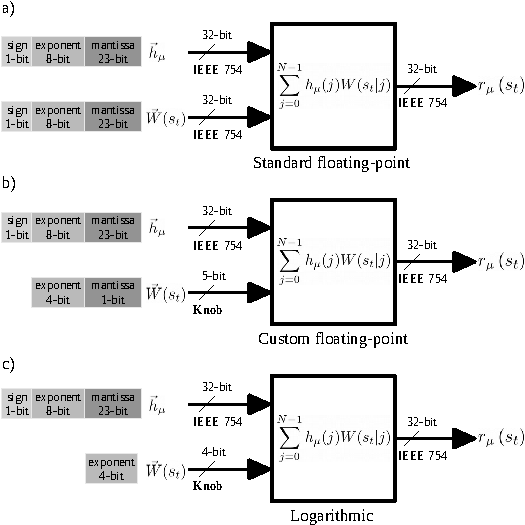
\includegraphics[width=\columnwidth]{../figures/dot-product_unit.pdf}
	\caption{Dot-product hardware module with (a) standard floating-point (IEEE 754) arithmetic, (b) hybrid custom floating-point approximation, and (c) hybrid logarithmic approximation.}
	\label{fig:dot_product_unit}
\end{figure}

Our main contributions are as follows:

\begin{itemize}
	\item We develop a hardware component for dot-product approximation. To perform the sum of pairwise products of two vectors, this hardware module has the following three design features: (1) the pairwise product is approximated by adding integer exponents and multiplying truncated mantissas, and the sum of products is done by accumulating denormalized integer products with barrel shifters, which increases computational throughput; (2) the synaptic weight vector uses either reduced custom floating-point or logarithmic representation, which reduces memory footprint; and (3) the neuron vector uses either standard or custom floating-point representation, which preserves QoR and overall inference accuracy.
	\item We address a design exploration with the proposed dot-product approximation using synaptic weight vectors with custom floating-point and logarithmic representation as shown in \fig{fig:dot_product_unit}. We evaluate inference latency, accuracy degradation, resource utilization and power dissipation. Experimental results demonstrate $20.5\times$ latency enhancement versus embedded CPU (ARM Cortex-A9 at 666MHz), and less than $0.5\%$ of accuracy degradation on a handwritten digit recognition task.
	\item We propose a noise tolerance plot as quality monitor, which serves as an intuitive visual model to provide insights into the accuracy degradation of SbS networks under approximate processing effects.
	\item Our proposed design for dot-product approximation is adaptable as a building block for other error-resilient applications (e.g., image/video processing).
\end{itemize}


The rest of the paper is organized as follows. Section~\ref{sec:related_work} covers the related work; Section~\ref{sec:background} introduces the background to SbS networks; Section~\ref{sec:system_design} describes the system design and the approximate dot-product hardware module; Section~\ref{sec:experimental_results} presents the experimental results thorough a design exploration flow; Section~\ref{sec:conclusions} concludes the paper.


To promote the research on SbS networks, our design exploration framework is made available to the public as an open-source project at http://www.ids.uni-bremen.de/sbs-framework.html

